%!TEX root = ../main.tex
\chapter{Transformada Watershed}
\label{chap:marco}
En este capítulo se definen los conceptos básicos de  ordenamiento vectorial y la matemática morfológica que serán utilizados posteriormente, así también la transformada de watershed por inundación y métodos de ordenes utilizados en este trabajo. 

\section{Matemática Morfológica}
La segmentación es el proceso de particionar imágenes digitales en múltiples segmentos. El objetivo de la segmentación es modificar y/o simplificar la forma en la que se representa una imagen, para que sea más significativa y fácil de analizar~\cite{wiki:segmentacion}. La matemática morfológica es una rama del análisis de imágenes basada en la teoría de conjuntos y principios algebraicos y geométricos~\cite{matheron2002birth}.

Los operadores básicos de la matemática morfológica son la erosión ($\varepsilon$) y la dilatación ($\delta$), que pueden ser definidos a partir del mínimo y el máximo respectivamente dentro de una ventana llamada elemento estructurante~\cite{noguera2014color}. 

Dada una ventana $E$, representada como el elemento estructurante, y una imagen $F$. 
\addsymbol{symbol:E} \addsymbol{symbol:F} 
\addsymbol{symbol:erosion} \addsymbol{symbol:dilatacion} \addsymbol{symbol:estructurante} 
La erosión ($\varepsilon$) de $F$ utilizando $E$ se puede definir como:
\begin{equation}
\varepsilon(F,E)(u,v)  = \min_{(i,j) \in E} \{F(u-i,v-j) + E(i,j) \},
\end{equation}
y la dilatación ($\delta$) de $F$ utilizando $E$ se puede definir como:
\begin{equation}
\delta(F,E)(u,v)  =  \max_{(i,j) \in E} \{F(u+i,v+j) - E(i,j) \}.
\end{equation}
\addsymbol{symbol:F}
\addsymbol{symbol:j}
La gradiente ($\gamma$) es el cambio direccional en la intensidad o color de una imagen. La gradiente ($\gamma$) es la resultante de la diferencia entre la dilatación ($\delta$) y la erosión ($\varepsilon$) de la imagen $F$~\cite{beucher}, se define como:
\begin{equation}
\gamma(F,E)(u,v) = \delta(F,E)(u,v) - \varepsilon(F,E)(u,v).
\end{equation}
\addsymbol{symbol:F}
\addsymbol{symbol:gradiente}
En escala de grises obtener la relación de orden entre los pixeles es trivial, debido a que están clasificados de acuerdo al orden natural de los valores que representan la intensidad de los píxeles. En imágenes a color los píxeles están representados por vectores. Un problema abierto es la extensión de la matemática morfológica para imágenes multivaloradas, como son las imágenes a color~\cite{aptoula2007}.
Los principales tipos de procesamiento morfológico para imágenes multivaloradas son~\cite{aptoula2007}:
\begin{itemize}
\item Procesamiento Marginal: en el procesamiento marginal cada canal es procesado de manera independiente y no existe la correlación entre los canales.
\item Procesamiento Vectorial: en el procesamiento vectorial se procesan todos los canales de manera conjunta. Se considera a los píxeles como vectores, y son tratados como una unidad de procesamiento. Requiere de un esquema de ordenamiento vectorial.
\end{itemize}

El procesamiento marginal tiene como principal desventaja la pérdida de información de la imagen al procesar por separado cada uno de los canales. Por otra parte, el procesamiento vectorial aprovecha dicha información obteniendo mejores resultados.
\section{Ordenamiento Vectorial}
La Matemática Morfológica requiere establecer una relación de orden entre los colores, representados por vectores, para ser extendida a color. 
En general, una relación binaria $\beta$ en un conjunto $D$ es:
\addsymbol{symbol:beta}\addsymbol{symbol:D}
\begin{enumerate}
\item Reflexivo si $\boldsymbol a \beta \boldsymbol a, \forall \boldsymbol a \in D$,
\item Anti-Simétrico si $\boldsymbol a \beta \boldsymbol b$ y  $\boldsymbol b \beta \boldsymbol a \Rightarrow \boldsymbol a = \boldsymbol b, \forall \boldsymbol a, \boldsymbol b \in  D$,
\item Transitivo $\boldsymbol a \beta \boldsymbol b$ y $\boldsymbol b \beta \boldsymbol c \Rightarrow \boldsymbol a \beta \boldsymbol c, \forall  \boldsymbol a, \boldsymbol b, \boldsymbol c \in D$,
\item Total si $\boldsymbol a \beta \boldsymbol b$ o $\boldsymbol b \beta \boldsymbol a, \forall \boldsymbol a, \boldsymbol b \in D$.
\end{enumerate}

La relación de orden $\leq$ (menor o igual) es requerida para la relación binaria $\beta$.
Cuando la relación de orden $\leq$ cumple con las restricciones 1 y 3 es llamada pre-orden. Una relación de orden es considerada como un ordenamiento si además de cumplir con las restricciones de una relación de pre-orden, también cumple con la restricción 2.
Adicionalmente a todo lo anterior, la relación $\leq$ debe cumplir la restricción 4 para ser considerado como orden total, sino es considerado como orden parcial.

Las técnicas de ordenamiento vectorial pueden ser clasificadas en los siguientes grupos~\cite{barnett1976ordering}:
\begin{itemize}
\item Ordenamiento Marginal (Ordenamiento M): Este ordenamiento cada componente compara el color de manera independiente.
\item Ordenamiento Condicional (Ordenamiento C): Un componente marginal es seleccionado secuencialmente para ordenar los vectores, dependiendo de las diferentes condiciones. Un ejemplo muy utilizado en el Ordenamiento C es el orden lexicográfico, que utiliza todos los componentes disponibles de los vectores a ser ordenados.
\item Ordenamiento Parcial (Ordenamiento P): Este ordenamiento esta basado en la división de los vectores en grupos de equivalencia, tal que entre los grupos existe un orden. Algunos ordenamientos totales son considerados dentro de esta clase.
\item Ordenamiento Reducido (Ordenamiento R): Los vectores son reducidos a valores escalares y posteriormente son clasificados mediante su orden escalar natural. Por ejemplo, un ordenamiento R en $\mathbb{Z}^{n}$ puede considerarse tras definir una transformación $T : \mathbb{Z}^{n} \rightarrow \mathbb{R}$ y posteriormente ordenar mediante orden escalar de su proyección en $\mathbb{Z}^{n}$ por $T$.
\begin{equation}
\forall q,q^{\prime}\in\mathbb{R}^{n} 
q \leq q^{\prime} \Leftrightarrow T\left(q\right) \leq T\left(q^{\prime}\right).
\end{equation}
\end{itemize}
\section{Ordenamientos}
\label{chap:marco}
A continuación se presentan los ordenamientos utilizados en este trabajo. Se utilizan píxeles $q$, $s$ y $t$ y sus respectivos componentes $(V_{1},V_{2},V_{3})$, $(V_{1},V_{2},V_{3})$ y $(V_{1},V_{2},V_{3})$ para ejemplificar el comportamiento de los ordenamientos que se explican posteriormente.

\subsection{Lexicográfico}
\label{chap:marco-lex}
El orden lexicográfico es también conocido como el orden de diccionario~\cite{chanussot1998total}~\cite{talbot98complete}. Una prioridad es asignada a cada componente del vector par que unos tengan mayor importancia que los otros al momento de realizar una comparación y definir un orden.
\addsymbol{symbol:q} \addsymbol{symbol:V}
\addsymbol{symbol:n} \addsymbol{symbol:lex}
\begin{equation}
q \leq q^{\prime} \Leftrightarrow \left[  V_{1},...,V_{n} \right]^{T} \leq_{L} \left[  V^{\prime}_{1},...,V^{\prime}_{n} \right]^{T},
\end{equation}
donde $\leq_{L}$ es el orden lexicográfico.

Para determinar si uno es mayor al otro se realiza los siguiente: se establece la prioridad entre los componentes, es decir, el componente $r$ tiene la mayor prioridad, luego el componente $g$ y por ultimo el $b$. Luego se compara inicialmente el primer componente con mayor prioridad, en caso de darse una igualdad, se compara el siguiente componente de mayor prioridad y así sucesivamente. De acuerdo a como se realice la selección de la prioridad, se podrían obtener resultados distintos.
\addsymbol{symbol:vec}
Por ejemplo, dados los píxeles $q=\left\{2,4,9\right\}, s=\left\{2,5,9\right\}, t=\left\{8,4,1\right\}$, se comparan los valores del componente con mayor prioridad, donde el componente $r$ tiene mayor prioridad, luego $g$ y $b$. Se puede observar que $t>s$ y $t>q$. No se puede determinar el orden entre $q$ y $s$, por lo cual se toma el siguiente componente con mayor prioridad, donde se puede observar que $t>s>q$.

\subsection{Alpha modulus lexicográfico}
\label{chap:marco-alphalex}
Una extensión del ordenamiento lexicográfico mostrado anteriormente fue propuesta en~\cite{angulo2003morphologie} que consiste en utilizar un valor $\alpha$ que el usuario defina, para modificar el grado de influencia que posee el primer componente. Se formula de la siguiente manera:
\addsymbol{symbol:q} \addsymbol{symbol:V}
\addsymbol{symbol:n} \addsymbol{symbol:lex}
\addsymbol{symbol:alpha}
\begin{equation}
q \leq q^{\prime} \Leftrightarrow \left[  \lceil V_{1}/\alpha\rceil , V_{2},...,V_{n} \right]^{T} \leq_{L} \left[  \lceil V^{\prime}_{1}/\alpha\rceil, V^{\prime}_{2},...,V^{\prime}_{n} \right]^{T}.
\end{equation}
\addsymbol{symbol:vec}
Por ejemplo, dados los píxeles $q=\left\{5,4,9\right\}, s=\left\{8,5,9\right\}, t=\left\{18,4,1\right\}$, se comparan los valores del componente con mayor prioridad dividido por el valor $\alpha$, donde se puede observar que $t>s$ y $t>q$, ya que $\lceil q_{1}/\alpha\rceil = 1,\lceil s_{1}/\alpha\rceil = 1,\lceil t_{1}/\alpha\rceil = 2$. No se puede determinar el orden entre $q$ y $s$, por lo cual se toma el siguiente componente con mayor prioridad, donde se puede observar que $t>s>q$.


\subsection{Vázquez et al}
\label{chap:marco-vazquez}
\addsymbol{symbol:T} \addsymbol{symbol:V} \addsymbol{symbol:w} \addsymbol{symbol:q}
\addsymbol{symbol:j} \addsymbol{symbol:F}
\addsymbol{symbol:n}\addsymbol{symbol:Sp}
\addsymbol{symbol:win}

Vázquez~\cite{noguera2014color} propuso una modificación del ordenamiento lexicográfico, tomando información de la imagen para obtener una transformación que se utiliza como el componente de mayor prioridad del orden lexicográfico.

La transformación propuesta por Vázquez en~\cite{noguera2014color} esta expresada como sigue: Para considerar la información local analizada por los operadores morfológicos, la imagen $F$ es particionada en ventanas denotadas por $win$, donde $win \subset F$. La transformada $T(q): \mathbb{Z}^{n}\rightarrow \mathbb{R}$ del píxel $q$ se obtiene mediante el producto escalar del vector $V = \left\{V_{1},V_{2},V_{3} \right\}$ correspondiente al píxel $q$ en el espacio de color $Sp$ con el vector de pesos $w = \left\{w1,w2,w3 \right\}$, es decir:
\begin{equation}
T\left(q\right) = \sum_{j=1}^n w_{j} \times V_{j}.
\end{equation}
\addsymbol{symbol:vec}
Por ejemplo, dados los píxeles $q=\left\{2,4,9\right\}, s=\left\{1,5,9\right\}, t=\left\{8,4,1\right\}$, utilizando la media en cada uno de los componentes, se forma el vector de pesos con los valores $w=\left\{5,6,9\right\}$, posteriormente se tienen los resultados:
$T(q)=2\times5+4\times6+9\times9=115,
T(s)=1\times5+5\times6+9\times9=116,
T(t)=8\times5+4\times6+1\times9=73$, donde se puede observar que $s>q>t$.

Las variaciones están dadas en el cálculo del vector de pesos $w$, para el cual se realizaron cálculos con la media, mínimo, máximo, entropia, moda, moda máximo, moda mínimo, suavidad y varianza de la imagen. Las comparaciones fueron realizadas en el espacio de color RGB para todas las variantes y se utiliza solo la transformada para la comparación debido a que para la transformada de watershed el hecho de que dos colores diferentes tengan la misma transformada no es un problema ya que se agruparán en el mismo nivel.

\subsection{Distancia euclidiana}
\label{chap:marco-distanciaeuclidianta}
Para el espacio de color RGB se realiza el cálculo con la distancia al origen, mientras que en el espacio de color CIELab se calcula con las distancias al origen, media y mediana de la imagen. 

Para el espacio de color CIELab se utiliza la fórmula descrita en \ref{formula:eucli}. Para el espacio de color RGB se utiliza la diferencia de color entre dos coordenadas $(r_{1},g_{1},b_{1})$ y $(r_{2},g_{2},b_{2})$ definido como $\Delta E_{rgb}$:~\cite{robertson1977cie}.
\addsymbol{symbol:r}\addsymbol{symbol:g}
\addsymbol{symbol:b}\addsymbol{symbol:ergb}
\begin{equation}
\label{formula:euclirgb}
\Delta E_{rgb} = \sqrt{(\Delta r)^2 + (\Delta g)^2 +(\Delta b)^2},
\end{equation}
donde 
\addsymbol{symbol:deltargbR}
\addsymbol{symbol:deltargbG}
\addsymbol{symbol:deltargbB}
\begin{equation}
\Delta r = r_{1} - r_{2},
\Delta g = g_{1} - g_{2},
\Delta b = b_{1} - b_{2}.
\end{equation}
\addsymbol{symbol:vec}
Por ejemplo, dados los píxeles $q=\left\{2,4,9\right\}, s=\left\{1,5,9\right\}, t=\left\{8,4,1\right\}$, utilizando la distancia al origen, se tienen los resultados:
$T(q)=\sqrt{(2-0)^{2}+(4-0)^{2}+(9-0)^{2}}=10.04$ ,
$T(s)=\sqrt{(1-0)^{2}+(5-0)^{2}+(9-0)^{2}}=10.34$ ,
$T(t)=\sqrt{(8-0)^{2}+(4-0)^{2}+(1-0)^{2}}=9$ , donde se puede observar que $s>q>t$.


\subsection{Entrelazado de bits}
\label{chap:marco-entrelazado}
El ordenamiento por entrelazado de bits consiste en una transformación inyectiva explotando la representación binaria de cada uno de los componentes, obteniendo un orden total en el espacio vectorial~\cite{chanussot1997bit}~\cite{chanussot1998total}.
Para un píxel $q$ con componentes ${x,y,z}$ en el espacio de color $Sp$, codificado en $k$ bits, la transformación por reducción $T: \mathbb{Z}^{n}\rightarrow \mathbb{Z}$ se calcula mediante la fórmula:
\addsymbol{symbol:q} \addsymbol{symbol:V}
\addsymbol{symbol:n} \addsymbol{symbol:k} 
\addsymbol{symbol:m} \addsymbol{symbol:T}
\addsymbol{symbol:j} \addsymbol{symbol:Sp}
\begin{equation}
T\left(q\right):\sum_{m=1}^k\left\{
2^{n.(k-m)}.\sum_{j=1}^n 2^{n-j}.V_{j,m}\right\},
\end{equation}
donde $V_{j,m}$ corresponde al m-ésimo bit del j-ésimo componente del píxel $q$. La representación binaria de $T(q)$ resultante se convierte en:
\begin{equation}
V_{1,1}V_{2,1}...V_{n,1}V_{1,2}V_{2,2}...V_{n,2}...V_{1,k}V_{2,k}...V_{n,k}.
\end{equation}
\addsymbol{symbol:vec}
Por ejemplo, dados los píxeles $q=\left\{2,4,9\right\}, s=\left\{1,5,9\right\}, t=\left\{8,4,1\right\}$, y la función de transformación T, los componentes expresados en 4 bits, se tienen los resultados:

$T(q)=\overbrace{0010}^2\overbrace{0100}^4\overbrace{1001}^9,
T(s)=\overbrace{0001}^1\overbrace{0101}^5\overbrace{1001}^9,
T(t)=\overbrace{1000}^8\overbrace{0100}^4\overbrace{0001}^1$, donde se puede observar que $t>q>s$.

\subsection{Ordenamiento utilizado por Meyer}
\label{chap:marco-meyer}
El ordenamiento de los píxeles utilizado en la propuesta de Meyer~\cite{Meyer} utiliza el espacio de color RGB. El mismo realiza una transformación por reducción a un valor escalar mediante la fórmula:
\addsymbol{symbol:r} \addsymbol{symbol:g}
\addsymbol{symbol:b} 
\begin{equation}
Max\left(|r_{s}-r_{t}|,|g_{s}-g_{t}|,|b_{s}-b_{t}|\right).
\end{equation}
Posteriormente el orden natural de los números es utilizado para realizar la comparación. Para la implementación se asume como píxel de referencia el origen $\left\{0,0,0\right\}$.
Por ejemplo, dados los píxeles $s=\left\{2,4,8\right\}, t=\left\{1,5,9\right\}$, se tienen los resultados:
$T(s)=Max\left(|2-0|,|4-0|,|8-0|\right)=8,
T(t)=Max\left(|1-0|,|5-0|,|9-0|\right)=9$, donde se puede observar que $t>s$. Podría darse el caso que para ambos píxeles se obtenga el mismo resultado, lo que haría que dos pixeles tengan la misma transformación y no se pueda determinar el orden entre $t$ y $s$.
\section{Algoritmo de watershed}
\label{chap:marco}

El algoritmo propuesto en este trabajo se basa en la implementación del algoritmo de Vincent y Soille~\cite{VincentSoille}, el cual propone un enfoque de crecimiento de regiones a partir de los mínimos locales. A continuación se muestra un ejemplo gráfico para mejorar el entendimiento. Se hace una analogía con la geografía como se muestra en la Figura \ref{img:relieve}(a). Cada uno de los relieves topográficos de la imagen son inundados con agua, donde las líneas watershed son las divisorias de distintos depósitos de agua~\cite{parwashed}. Las entradas del algoritmo son la gradiente morfológica de la imagen y los marcadores. La transformación watershed puede ser clasificada bajo el enfoque de segmentación basado en regiones. 

El algoritmo de watershed en escala de grises descrito por Vincent y Soille~\cite{VincentSoille} realiza una inundación por niveles, desde el mínimo hasta el máximo nivel de intensidad de los píxeles de la imagen. En las Figuras \ref{img:relieve}(b),(c) y (d) se muestra como se van inundando los niveles. Las zonas de baja intensidad se conocen como vasijas (basins en Inglés), por donde fluirá el agua e inundará toda la imagen; es decir, el agua fluirá en cada una de las vasijas identificadas a partir de los mínimos de la imagen. El proceso de inundación continúa hasta que las aguas de cuencas o vasijas contiguas se unan, formando líneas de unión que representarán las fronteras de regiones homogéneas, y constituyen el resultado de la segmentación~\cite{parwashed}, como se muestra en la Figura \ref{img:relieve}(e). El crecimiento de regiones se inicia a partir de marcadores obtenidos por la selección de todos los mínimos del gradiente, lo que podría producir una segmentación no deseada. En la Figura \ref{img:relieve}(e) se muestra como el objeto segmentado fue dividido en el medio, produciendo un resultado no deseado.
\begin{figure}[H]
\centering
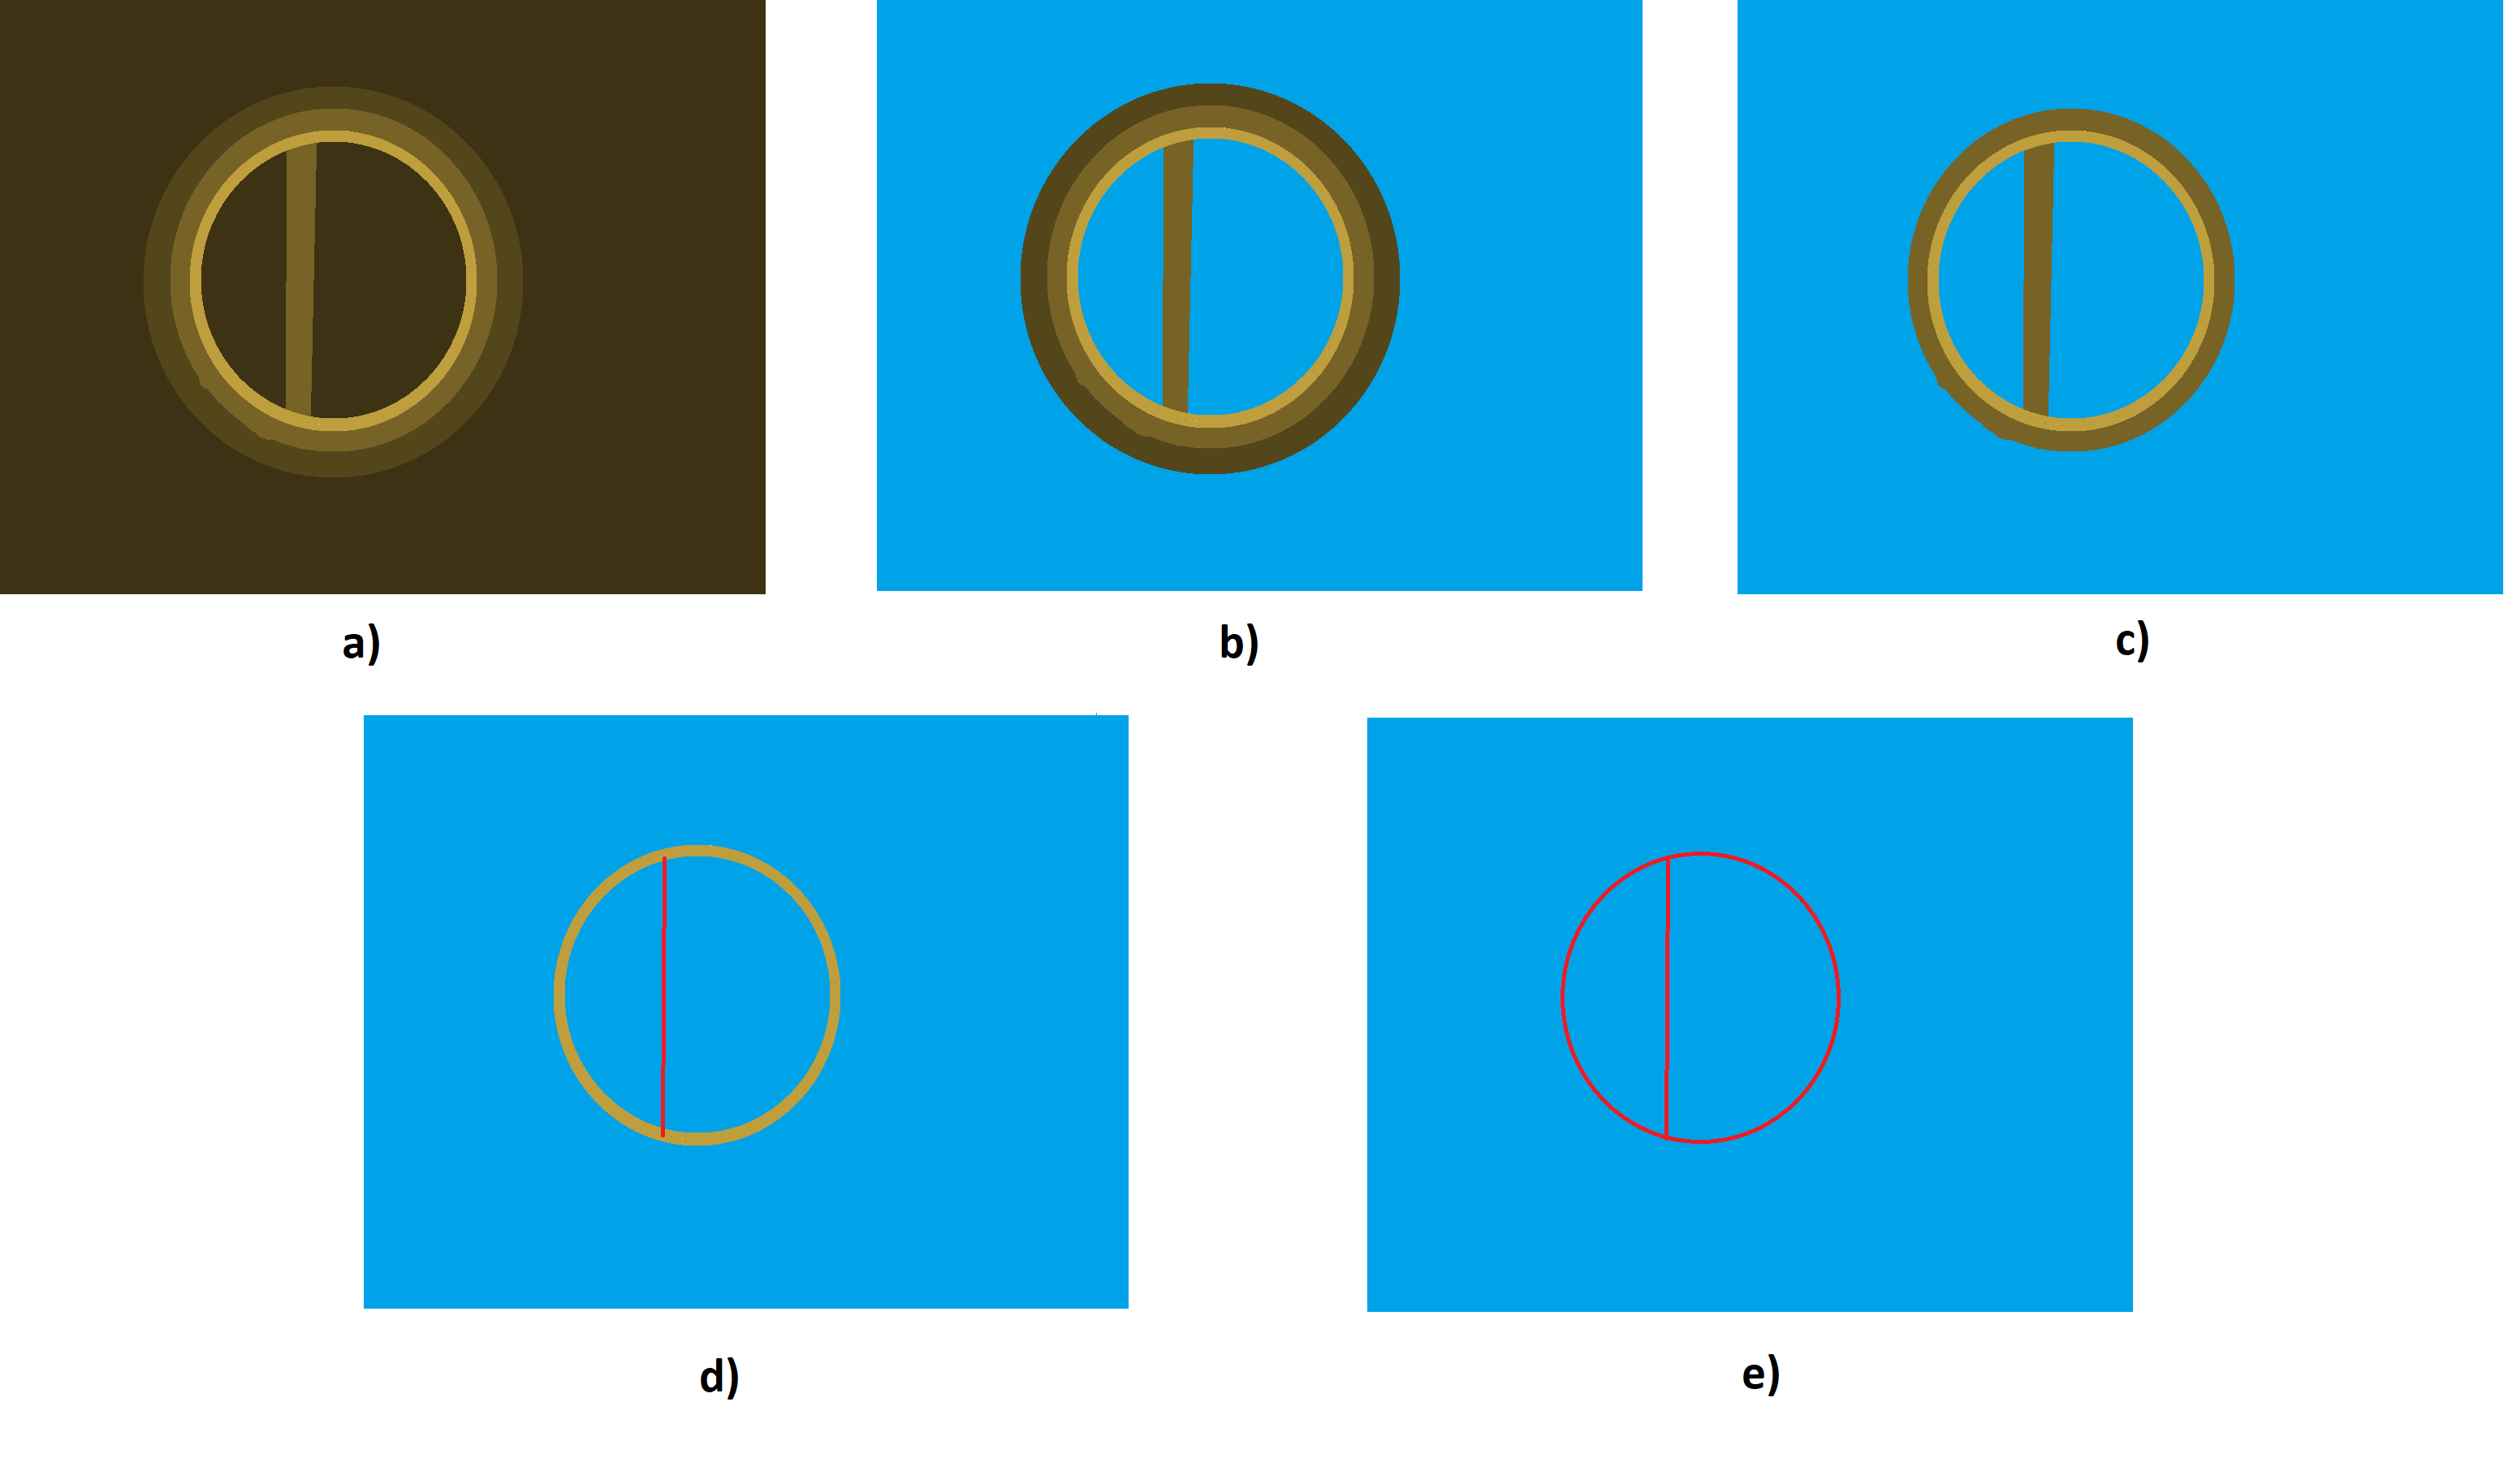
\includegraphics[width=150mm]{./imagenes/sin_marcadores.png}
\caption{Proceso de inundación con resultados no deseados}
\label{img:relieve}
\end{figure}

Al momento de la inundación, se tiene en cuenta una relación de orden dual entre los píxeles a ser inundados. La relación dual se entiende como la dependencia que existe entre dos criterios de ordenamiento, el orden de llegada a la cola y la altura de los píxeles. Un píxel de menor altura se debe inundar primero, así también los vecinos que se encuentren en una misma altura deben ser inundados antes de seguir con el orden anterior. Un algoritmo que simule la inundación tiene que poder reproducir la relación de orden dual, que naturalmente se obtiene con el uso de una cola de prioridad. Una cola de prioridad permite almacenar puntos en cualquier orden y devolverlos en el orden de la inundación.

El proceso de watershed para imágenes cromáticas puede afrontarse desde diversos enfoques. El empleo de información cromática en el proceso de watershed es posible por ejemplo, calculando el watershed en cada una de las señales cromáticas y combinar después los resultados~\cite{Saarinen}. Otra posibilidad es calcular el watershed directamente sobre la imagen a color~\cite{Meyer}.

La transformación watershed permite calcular los contornos más relevantes de la imagen, pudiendo así seleccionar los resultados deseados~\cite{Meyer}. En algunos casos donde las imágenes en escala de grises no presentan grandes variaciones de intensidad entre diferentes cuerpos, podría obtenerse una segmentación no esperada. Considere la misma imagen pero esta vez a color, podría tener los mismos niveles de intensidad pero en diferentes canales, en cuyo caso visualmente se distingue de manera fácil la diferencia entre diferentes cuerpos. El color es una propiedad distinguible entre diferentes regiones de una imagen por lo cual una segmentación a color puede tener mejores resultados que una en escala de grises~\cite{Lezoray}.

\subsection{Marcadores}
Generalmente los puntos iniciales de la inundación son mínimos locales y los marcadores denotan la cantidad de regiones a ser obtenidas luego del proceso de segmentación. En algunas imágenes se tiene la presencia de un gran número de mínimos locales, produciéndose sobre-segmentación en pequeñas regiones. Muchas de las regiones generadas no son importantes dentro de la imagen, o no representan objetos existentes en la imagen original.

La sobre-segmentación se puede disminuir utilizando métodos de mejora como filtros morfológicos. Además de ellos se podrían aplicar otras formas para evitar la sobre-segmentación, como es la selección de marcadores. Seleccionar marcadores en la imagen resuelve dicho problema iniciando el proceso de inundación desde los píxeles marcados, que representan los objetos deseados a segmentar en la imagen~\cite{Yang}. En este trabajo los marcadores fueron seleccionados manualmente.

La imagen que se muestra en la Figura \ref{img:relieve1}(a) contiene un objeto circular que se desea segmentar. Para evitar una segmentación no deseada fueron seleccionados dos marcadores, uno dentro del objeto deseado y otro en el fondo de la imagen, como se muestra en la Figura \ref{img:relieve1}(b). Posteriormente se inicia el proceso de inundación a partir de los marcadores como se muestra en las Figuras \ref{img:relieve1}(c), (d) y (e). En la Figura \ref{img:relieve1}(f) se muestra el resultado de la segmentación del objeto deseado.


\begin{figure}[H]
\centering
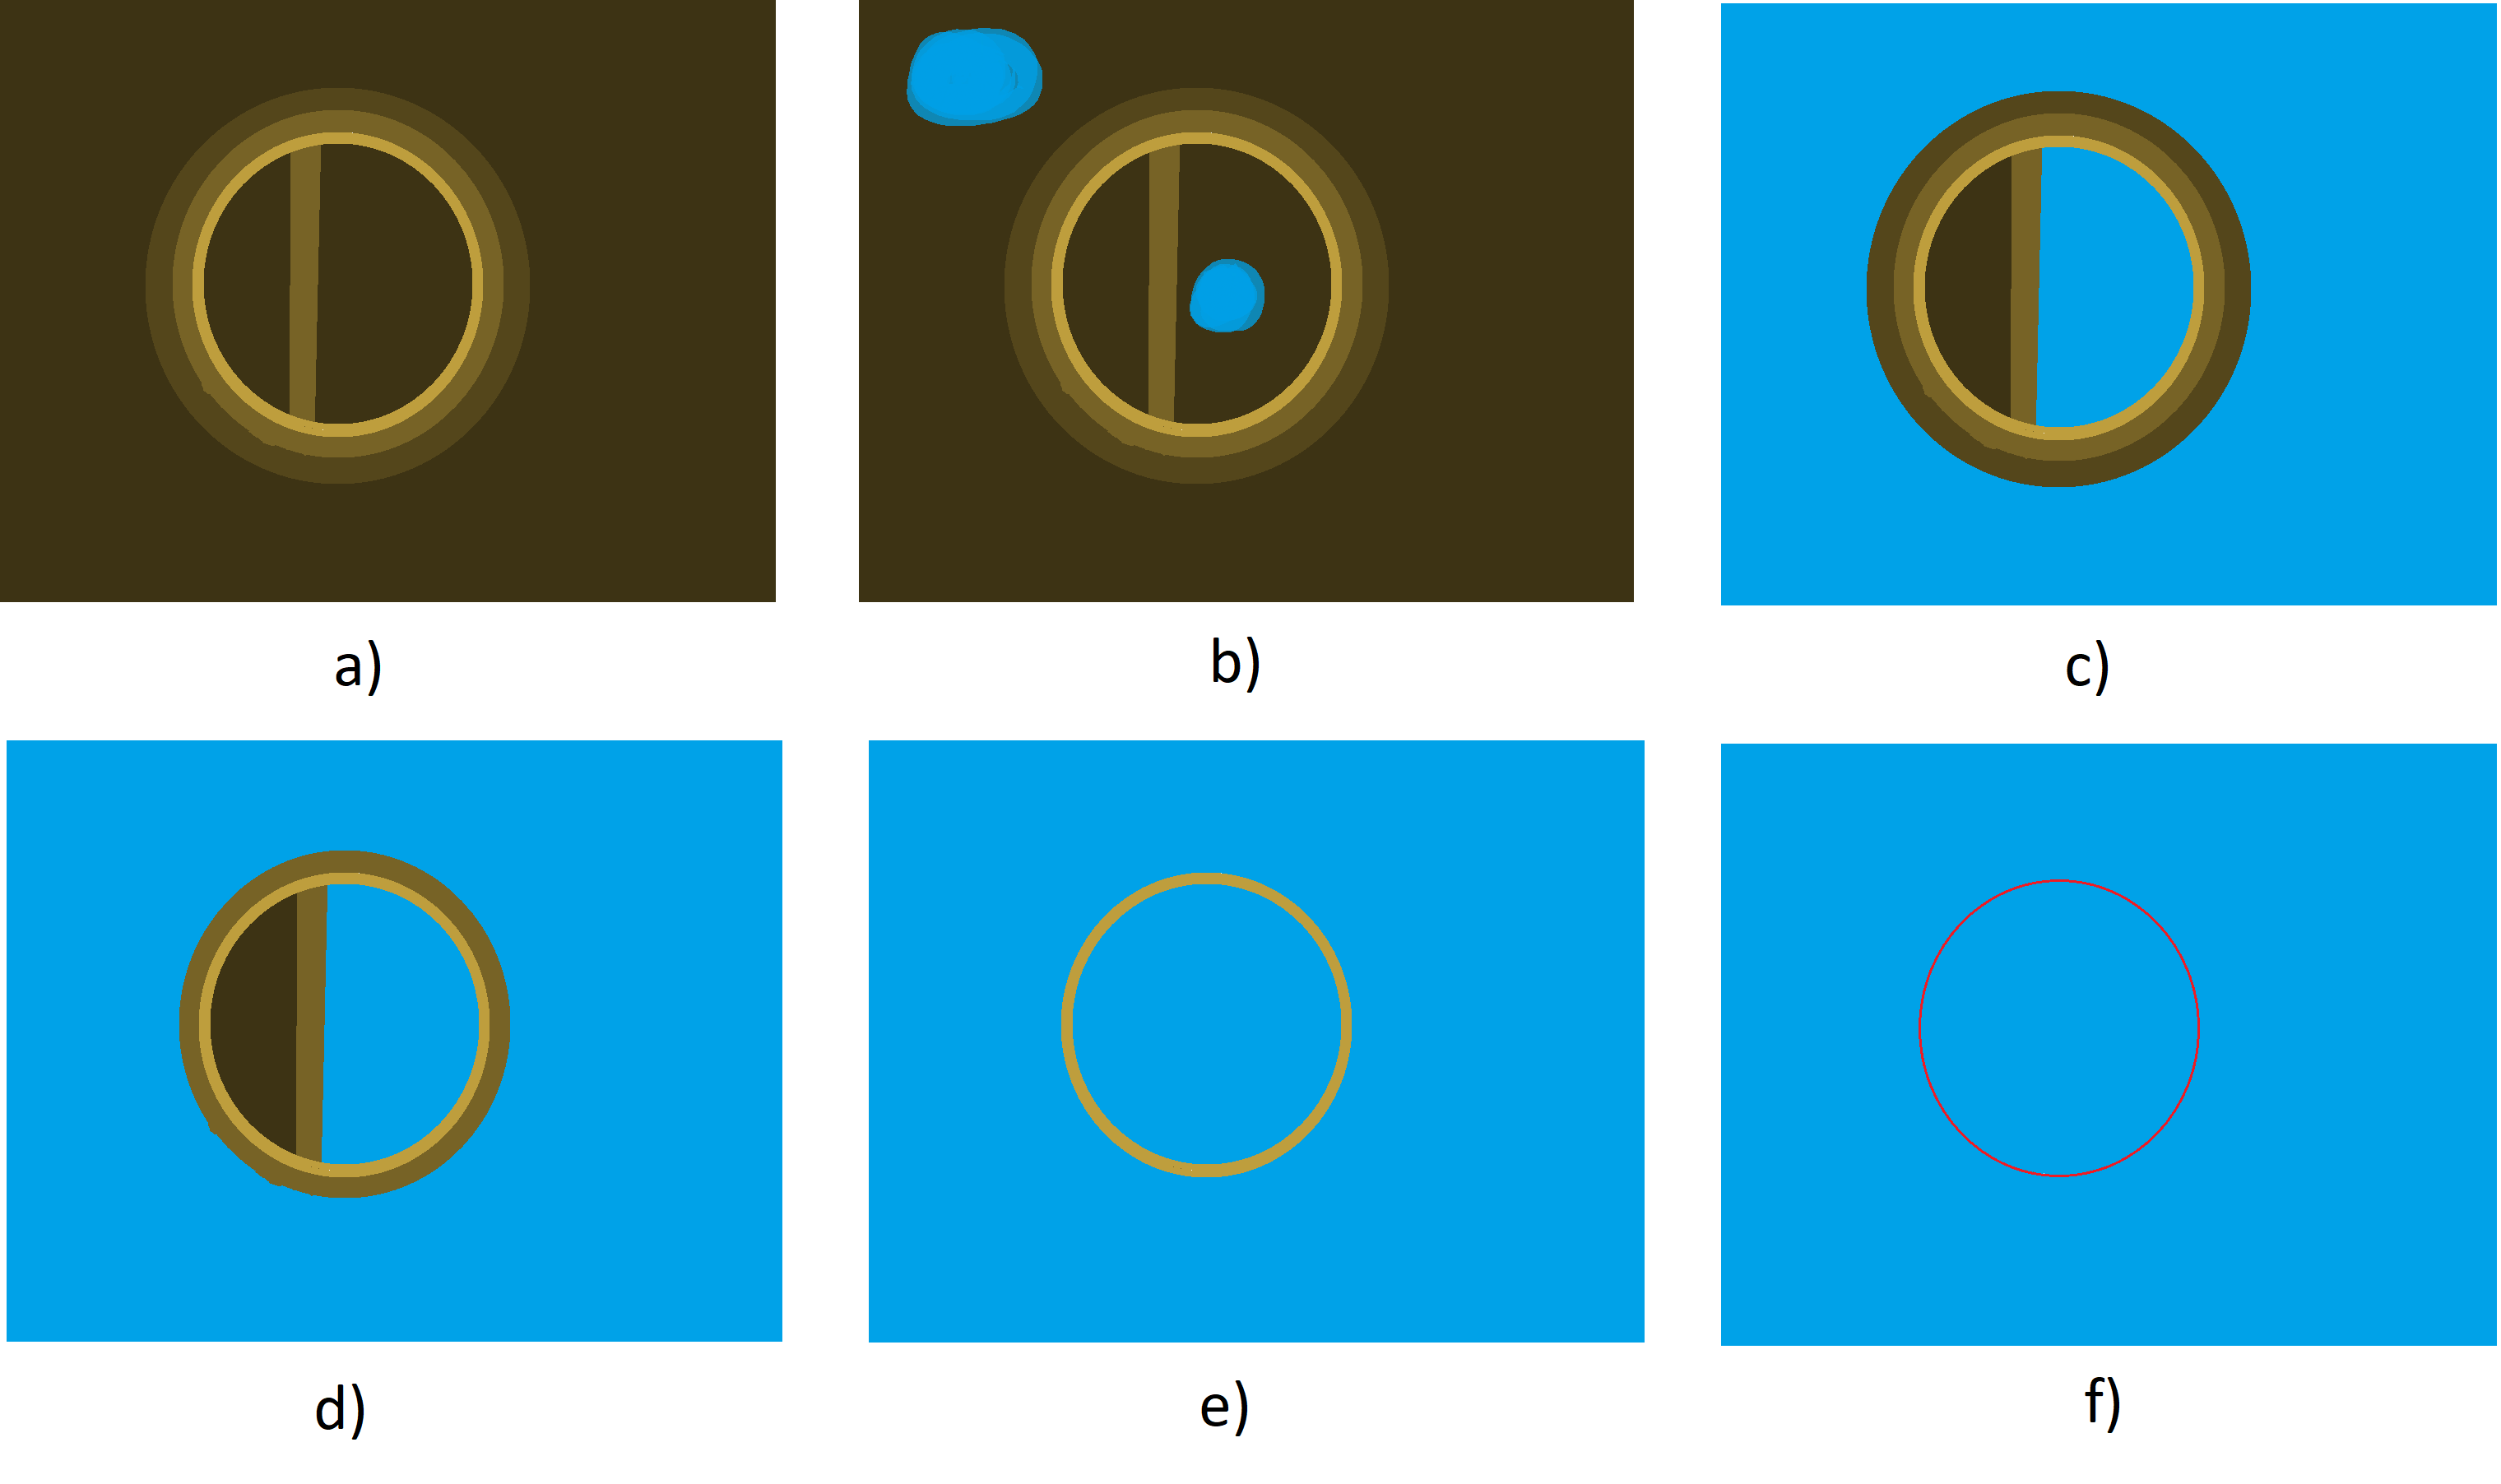
\includegraphics[width=140mm]{./imagenes/con_marcadores.png}
\caption{Proceso de inundación con marcadores del objeto deseado}
\label{img:relieve1}
\end{figure}



\section{Resumen}

En este capítulo se presentan los conceptos de:
\begin{itemize}
\item Segmentación
\item Operaciones básicas de matemática morfológica
\item Dilatación
\item Erosión
\item Gradiente morfológica
\item Criterios de ordenación de colores
\item Trasformada de watershed sin marcadores
\item Sobre-segmentación
\item Trasformada de watershed con marcadores
\end{itemize}
Se ejemplifica el proceso de inundación con y sin marcadores.
